\chapter{\fancyname{SessionTS}: Session Type API Generation for TypeScript}
\label{chap:codegen}

In this chapter, we present
\fancyname{SessionTS}, an API generation toolchain for building
web applications in TypeScript that conform to a communication protocol 
based on multiparty session type theory.

\fancyname{SessionTS} supports communication protocols that define 
\emph{server-centric} topologies, meaning that: 
\textbf{(1)} there is exactly one participant executed on the 
Node.js runtime; 
\textbf{(2)} all other participants run on the web browser; and
\textbf{(3)} all non-server participants only communicate with the server.
We relax this assumption in \cref{part:general}.

The toolchain is publicly available at \cite{repo}.

\section{Development Workflow}

We motivate our development workflow from previous work 
\cite{PureScript2019} by extending the Scribble toolchain
and generating APIs that integrate the developer's 
application logic
into the execution of the communication automata.

We visualise the workflow in \cref{fig:devworkflow} 
and provide a brief overview:

\begin{enumerate}

\item The developer supplies the communication protocol written in
Scribble (\cref{subsection:scribble}), 
stating the role (hereafter \textit{endpoint})
to generate APIs for,
and the code generation \textit{target} 
(i.e. whether the role runs on the server or the web browser).

\item \fancyname{SessionTS} delegates to the 
Scribble toolchain for verifying the well-formedness of
the protocol and expects to receive a DOT graph representation of
the endpoint FSM (\cref{subsection:efsm}). 
\fancyname{SessionTS} parses the endpoint's 
interactions from the DOT graph and generates TypeScript APIs
for the developer (\cref{subsection:apigen}) 
tailored to the specified target.

\item The developer implements their web application using the
generated APIs. Implementations that pass the type-checking phase
of the TypeScript Compiler are guaranteed to be free from 
communication errors by session type theory.

\end{enumerate}

\begin{figure}[!ht]
\centering
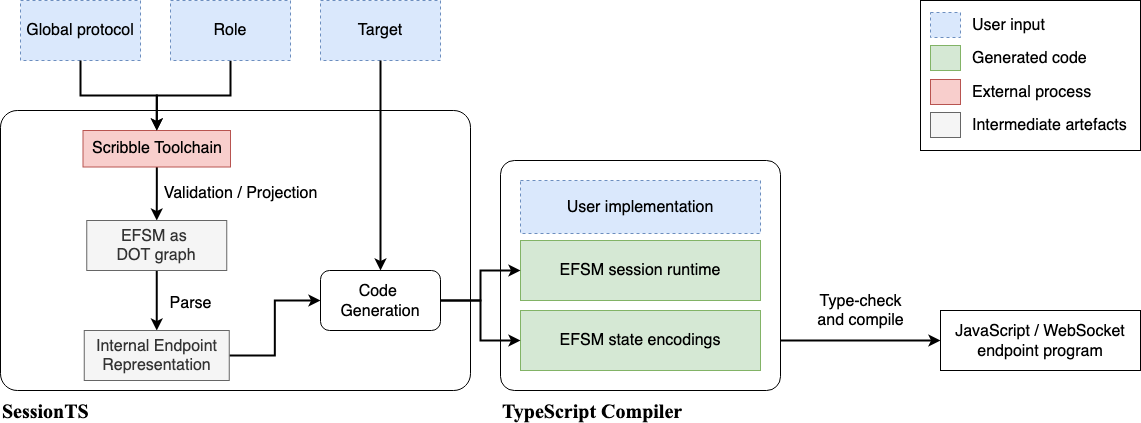
\includegraphics[width=\textwidth]{DevelopmentWorkflow}
\captionof{figure}{Overview of \fancyname{SessionTS} Development Workflow}
\label{fig:devworkflow}
\end{figure}

\subsection{Protocol Specification with Scribble}
\label{subsection:scribble}

We use the Scribble protocol description language, 
as presented in
\cite{Scribble}, for formalising the communication structure. This is
inspired by existing work on implementing session type theory 
in mainstream programming languages
\cite{Hybrid2016, PureScript2019, Python2017}. 
We use the variant of the Scribble language 
previously introduced in \cref{subsection:bgscribble}.

\subparagraph{Type declaration statements}
Specific to our TypeScript API generation toolchain,
the developer is \textit{not} required to explicitly
add type declaration statements for built-in types.
\cref{lst:adder} is a \textit{syntactically correct}
Scribble protocol as far as 
\fancyname{SessionTS} is concerned. 
Internally, \fancyname{SessionTS} inspects the protocol file
and parses existing type declarations using regular expressions
(or \textit{regex}) -- this is necessary to extract any
custom data types that will appear in the communication (for example,
\cref{lst:game}), and allows \fancyname{SessionTS} to inject
``boilerplate'' type declarations for built-in TypeScript types before
calling Scribble.

\begin{figure}[!ht]
\begin{lstlisting}[language=Scribble]
module Adder;

global protocol Adder(role Client, role Svr) {
	choice at Client {
		ADD(number, number) from Client to Svr;
		RES(number)         from Svr to Client;	
	} or {
		QUIT(string) from Client to Svr;	
		TERMINATE()  from Svr to Client;
	}
}
\end{lstlisting}
\captionof{lstlisting}{The \tprotocol{Adder} Protocol}
\label{lst:adder}
\end{figure}

We will use the \tprotocol{Adder} protocol as a running example
to demonstrate how our work performs TypeScript API generation.

\subsection{From Scribble to EFSM}
\label{subsection:efsm}

Given the protocol and endpoint, we use Scribble
to validate the well-formedness of the protocol and extract
information from the protocol relevant for the endpoint.
The latter is expressed as a finite state machine
where each state restricts the possible transitions, 
and transitions between states are represented by
communication actions, i.e. the sending or receiving of a message.

Scribble expresses the EFSM using the 
DOT graph description language \cite{dot}, with each
communication action encoded as the label of the corresponding
state transition. 
\fancyname{SessionTS} uses the pydot library \cite{pydot}
to parse the graph into an internal representation of the EFSM.
We define an \texttt{EfsmBuilder} class with APIs designed for
constructing the EFSM representation by iterating over the 
state transitions from the DOT representation.

\begin{figure}[!ht]
\begin{lstlisting}[language=Python]
@dataclass
class Endpoint:
    protocol: str
    role    : str
    server  : str
    efsm    : EFSM
    types   : typing.Iterable[DataType]
\end{lstlisting}
\captionof{lstlisting}{The Endpoint API}
\label{lst:endpointapi}
\end{figure}

As the code generation process requires additional information,
we define an \texttt{Endpoint} dataclass\footnote{
A Python dataclass uses the decorator to generate
``boilerplate'' methods, such as the constructor, based on the
properties listed in the annotations.} (\cref{lst:endpointapi})
to contain the \texttt{EFSM}
representation, along with the information passed in from the
command line (\texttt{protocol}, \texttt{role}, \texttt{server}) 
and the custom type declarations (\texttt{types}) parsed from the
protocol specification.

\subsection{API Generation}
\label{subsection:apigen}

Formally, API generation is a function of the constructed
\texttt{Endpoint} instance
\textit{and} the target specified in the command line. We use a 
different code generation strategy for implementations running on
the servre (\cref{chap:node}) versus the browser (\cref{chap:react}).
In this subsection, we explain how we perform API generation
at a higher level of abstraction.

Traditional methods of code generation involve applying the
Visitor pattern on the internal representation. 
In the context of the MPST framework,
this may involve defining a Visitor class that implements a
\texttt{generate()} operation to be performed on the EFSM states,
such that the \texttt{generate()} implementation specialises to the
type of EFSM state, i.e. send, receive or terminal.
This is not straightforward in Python, as method overloading is not 
supported, so the ``visit'' methods would need different names.
More importantly, it is less straightforward to visualise
the structure of the generated code, as the string interpolation
aspect is likely to be interleaved with source code implementing
additional logic for code generation.

For \fancyname{SessionTS}, we leverage the Jinja \cite{jinja} 
template engine library for code generation. 
We first construct templates for the TypeScript files we wish to generate,
specifying placeholders for dynamic content (to be extracted
from the \texttt{Endpoint} object); 
we then provide Jinja with the template path and the 
\texttt{Endpoint} object, and the template engine renders the
TypeScript code by filling in the dynamic placeholders. 
We show an example in \cref{lst:jinja}.

\begin{figure}[!ht]
\begin{lstlisting}[language=javascript, title=efsm.ts.j2]
export namespace Message {

  
  export type S{{ state ~ action.label }} = {
    label: Labels.S{{ state }}.{{ action.label }},
    payload: [{{ action.payloads|join(', ') }}],
  };
  
  export type S{{ state }} = 
  | S{{ state ~ action.label }};

\end{lstlisting}
\captionof{lstlisting}{Example Jinja Template for
\fancyname{SessionTS} API Generation}
\label{lst:jinja}
\end{figure}

Jinja provides lightweight syntax for injecting content and
markup for simple control structure: \texttt{\{\{ state \}\}} 
denotes a placeholder for Jinja to render the \texttt{state} variable,
and the \texttt{\{\% \%\}} syntax  is used for conditionals and
control structures 
(such as for loops, to dynamically render the enclosing ``sub-template''
by iterating over a collection).
The main advantage that Jinja brings is that 
it decouples the ``presentation''
from the ``content'' and makes it quick to prototype and extend
the generated code, \textit{usually} without modifications to the 
code generator.

\begin{figure}[!ht]
\begin{lstlisting}[language=python]
class CodeGenerationStrategy(ABC):

    target_to_strategy = {} (*@\label{line:mapping}@*)

    def __init__(self):
        super().__init__()

    @classmethod
    def __init_subclass__(cls, *, target):
        CodeGenerationStrategy.target_to_strategy[target] = cls (*@\label{line:register}@*)
        return super().__init_subclass__()
    
    @abstractmethod
    def generate(self, endpoint: Endpoint):
        pass
\end{lstlisting}
\captionof{lstlisting}{Implementing \texttt{CodeGenerationStrategy}}
\label{lst:codegenerationstrategy}
\end{figure}

As we generate a different set of TypeScript artefacts depending
on the specified target, we structure the different code generators
using the Strategy design pattern. Each target extends the
abstract base class \texttt{CodeGenerationStrategy} 
and implements its own \texttt{generate()}
method to return a list of \texttt{(path, content)} tuples. 
We define a \texttt{CodeGenerator} class that is parameterised 
by \texttt{target}: when instantiated, it will select and perform 
the specialised \texttt{generate()} method based on \texttt{target}, 
before formatting and committing the generated code 
to the file system.
We implement a subclass hook in \texttt{CodeGenerationStrategy}
(\cref{lst:codegenerationstrategy}),
such that each derived class must provide the target name to
``register'' with the base class (\cref{line:register}),
and the base class keeps an internal
mapping of the concrete strategies (\cref{line:mapping}); 
\texttt{CodeGenerator} accesses
this mapping to select the appropriate strategy.


\section{Protocol Specification with \fancyname{Scribble}}

\begin{itemize}
\item see notes from PLACES paper on scribble
\item scribble language definition (unless already in background)
\end{itemize}

\section{EFSM Encoding}
\label{section:nodeefsm}

We show the structure of the generated EFSM.ts file in
\cref{lst:nodeefsmfile}.
Note that the formal definition of the EFSM in 
\cref{section:scribbleefsm}
contains more than just states and the state transition function,
so we encode the additional information as well.
Each type of information is grouped into their own
\textit{namespace}, and are collectively exported in
the EFSM \textit{module} for the developer to use.

\begin{figure}
\begin{lstlisting}[language=javascript,tabsize=2,title=EFSM.ts]
// (*@\cref{subsection:nodeefsmroleslabelsmsg}@*)
export namespace Roles {...};
export namespace Labels {...};
export namespace Message {...};

// (*@\cref{subsection:nodeefsmhandlers}@*)
export namespace Handler {...};

// (*@\cref{subsection:nodeefsmimplementation}@*)
abstract class ISend {...};
abstract class IReceive {...};
abstract class ITerminal {...};
export namespace Implementation {...};

export type EfsmTransitionHandler =
	(implementation: Implementation.Type) => void;
export type MessageHandler = (message: any) => void;
\end{lstlisting}
\captionof{lstlisting}{Structure of Generated EFSM Encoding 
for Server Endpoint}
\label{lst:nodeefsmfile}
\end{figure}

\subsection{Roles, Labels, Messages}
\label{subsection:nodeefsmroleslabelsmsg}

We generate TypeScript constructs for these pieces of information
so they can be reused throughout the generated code, 
and in particular, the runtime.

\subparagraph{Roles}
The runtime needs to know the identifiers of participants involved
in the session, and who to send/receive from 
depending on the EFSM state.
We generate string enumerations, or \textit{enums}, for each 
participant in the protocol, \textit{excluding} the 
first person endpoint. 
The enum appropriately groups the collection
of participants involved and scales for multiparty sessions,
whilst making it simple to derive other types, e.g. a mapping from
participants (indexed by the enum) to WebSockets.

\subparagraph{Labels}
The runtime needs to decide which handler to invoke, based
on the label of the received message. Similarly, the developer needs
to provide handlers specifying their internal choice (e.g. which
message label to send) and how to handle external choice (e.g. 
how to handle received message with particular label).
For the same reason, we also generate string enums for message labels,
one enum per state. Enums are compatible with switch statements,
which can be used to dispatch messages to the correct handlers
in the runtime based on the message label. 
We give an example in \cref{lst:nodeefsmlabels}.

\begin{figure}[!ht]
\begin{lstlisting}[language=javascript,tabsize=2]
// Inside the Labels namespace...
export enum S51 { ADD = "ADD", QUIT = "QUIT", };
export enum S53 { RES = "RES", };
export enum S54 { THANKS = "THANKS", TERMINATE = "TERMINATE", };
\end{lstlisting}
\captionof{lstlisting}{Generated Label Enums for \trole{Svr} endpoint}
\label{lst:nodeefsmlabels}
\end{figure}

\subparagraph{Messages}
The handler APIs that we generate for developers
need to refer to the label identifier and payload type: 
we refer to this as the message structure, and encode this as a
Message Type. 
Each message is expressed as an interface with
properties for the label and payload.
These interfaces are grouped based on the EFSM state
they belong using \textit{union types}.
We illustrate this in \cref{lst:addersvrmsg}.
By expressing the payload type as a \textit{tuple}\footnote{
In TypeScript, a tuple is an array with fixed size
and known types for elements at each position.
},
we easily generalise our type definition to polyadic payloads.

\begin{figure}[!ht]
\begin{lstlisting}[language=javascript, tabsize=2]
// Inside the Message namespace...
export interface S54THANKS {
	label: Labels.S54.THANKS,
	payload: [string],
};
export interface S54TERMINATE {
	label: Labels.S54.TERMINATE,
	payload: [],
};

export type S54 = | S54THANKS | S54TERMINATE;
\end{lstlisting}
\captionof{lstlisting}{Generated Message Type Definition for State 54}
\label{lst:addersvrmsg}
\end{figure}

\subsection{Handler APIs}
\label{subsection:nodeefsmhandlers}

We collect the APIs that the developer needs to implement
under the \texttt{Handler} namespace. 
As a design choice, we \textit{do not} generate handlers for
terminal states, because the semantics of inactivity mean
there is nothing to handle.
We introduce the generated handlers for sending and receiving states.
These are non-terminal states that will involve the encoding of its
successor state. The reader will notice that, in the listings below,
the successor state is stated to be under the
\texttt{Implementation} namespace: we explain in 
\cref{subsection:nodeefsmimplementation}, but for now,
it is sufficient to acknowledge that those refer to the encoding
of the successor state.

\subparagraph{Send}
We model selections using a union type to
encapsulate the possible send actions, as shown in 
\cref{lst:addersvrsendhandler}.
Each send action is encoded as a tuple of
the label, the payload, and the successor state encoding.
We see some benefits from defining Message Types as interfaces:
TypeScript supports \textit{index type queries} to extract
named property types, so
\lstonelinejs{Message.S54THANKS['payload']} 
would resolve to \lstonelinejs{[string]},
based on the interface definition \cref{lst:addersvrmsg}.

\begin{figure}[!ht]
\begin{lstlisting}[language=javascript, tabsize=2]
// Inside the Handler namespace...
export type S54 = 
	| [Labels.S54.THANKS, Message.S54THANKS['payload'],
			Implementation.S52] 
	| [Labels.S54.TERMINATE, Message.S54TERMINATE['payload'], 
			Implementation.S52];
\end{lstlisting}
\captionof{lstlisting}{Generated Type for \trole{Svr} Send State
in \tprotocol{Adder} protocol}
\label{lst:addersvrsendhandler}
\end{figure}

We generalise deterministic send actions as a trivial \textit{selection}, 
as motivated from the theory (\cref{fig:globaltypes}),
so the encoding for State 53 in the \trole{Svr} FSM would be
the union of a single tuple.

\subparagraph{Receive}
We model branching using an interface to 
enumerate the possible branches, as shown in
\cref{lst:addersvrreceivehandler}.
As with send states,
we generalise deterministic receive actions as a trivial \textit{branch},
which would be an interface with one property. 

\begin{figure}[!ht]
\begin{lstlisting}[language=javascript,tabsize=2]
// Inside the Handler namespace...
export type S51 = {
	[Labels.S51.ADD]: (...payload: Message.S51ADD['payload']) =>
		Implementation.S53,
	[Labels.S51.QUIT]: (...payload: Message.S51QUIT['payload']) => 
		Implementation.S54,
}
\end{lstlisting}
\captionof{lstlisting}{Generated Type for \trole{Svr} Receive State
in \tprotocol{Adder} protocol}
\label{lst:addersvrreceivehandler}
\end{figure}

The interface properties are defined by the 
labels of the permitted receive actions:
the square-bracket notation means that the property name
is derived from the value of the enclosing variable,
so \lstonelinejs{[Labels.S51.ADD]} resolves to the
\lstonelinejs{'ADD'} string. 

The interface values are functions parameterised by
the message payload, and must return the successor state encoding.
We see another benefit of defining the payload in Message Types
as a tuple: we can define the receive handler parameter
using the \textit{spread syntax}, which allows the tuple
expression to be expanded into a list of function arguments. 
More concretely, as shown in \cref{lst:nodeefsmspread},
it allows the developer to pattern match on the
individual payload values (\cref{line:yesspread}) 
rather than defining their function to expect a tuple 
and manually destructing it (\cref{line:nospread}),
so the former is more intuitive.

\begin{figure}[!ht]
\begin{lstlisting}[language=javascript,tabsize=2]
const withSpread = (x: number, y: number) => {...} (*@\label{line:yesspread}@*)
const withoutSpread = (payload: [number, number]) => {...} (*@\label{line:nospread}@*)

const handler1: Handler.S51 = { ADD: withSpread		, ... };	// OK
const handler2: Handler.S51 = { ADD: withoutSpread, ... };	// OK
\end{lstlisting}
\captionof{lstlisting}{Example Handler Signature 
Compatible with Spread Syntax}
\label{lst:nodeefsmspread}
\end{figure}

\subsection{Wrapping Handlers in ``Implementations''}
\label{subsection:nodeefsmimplementation}

The behaviour of the runtime is dependent on the current state,
so it needs a way to distinguish between
all the different states -- one can think of this as implementing
the state transition function from the theory, which is analogue to 
overloading a \texttt{next()} method for each state.
Due to limitations in the TypeScript language, this would have to
be some sort of switch statement, with the \texttt{next()}
method parameterised by some base type assignable to all states.
Currently, the state is only determined by the handler
to be implemented by the developer, so the switch statement
and base type would have to be defined on the handler APIs.

Unfortunately, this is not practical. 
Handlers for send states are union types and
handlers for receive states are interfaces,
both of which are not supported 
by the \lstonelinejs{instanceof}
operator.

\subsubsection{Distinguishing Handlers using Conditional Types}

We attempt to address this by defining an enum of state identifiers
for each type of state (i.e. an enum for send states, 
an enum for receive states)
upon which to execute the EFSM, which solves the switch statement
problem.
Now, we are left with defining a mapping between the 
state identifier enum to the handler type. This construct would be
analogue to \textit{dependent types}, which again, is not a feature
of the TypeScript type system.

We try to define type dependencies using
\textit{conditional types} in TypeScript.
A conditional types is a type-level expression
\begin{lstlisting}[language=javascript,numbers=none]
T extends U ? X : Y;
\end{lstlisting}
which reads, \textit{if \texttt{T} is assignable to \texttt{U},
then the type is \texttt{X}; otherwise, the type is \texttt{Y}}.

Combined with \textit{generic constraints}\footnote{
\lstonelinejs{<T extends U>} defines a generic type \texttt{T}
and enforces that it must be a type assignable to \texttt{U}.
},
we can approximate the dependency between the state identifier
enum and the generated handler API using something
similar to \cref{lst:conditionaltypes}.

\begin{figure}[!h]
\begin{lstlisting}[language=javascript,tabsize=2]
enum SendState { S1, S3, ... };
enum ReceiveState { S2, S4, ... };
type State = SendState | ReceiveState;

type SendHandler<S extends SendState> = 
	S extends SendState.S1 ? Handler.S1 :
	S extends SendState.S3 ? Handler.S3 : ... ;

type ReceiveHandler<S extends ReceiveState> = 
	S extends ReceiveState.S2 ? Handler.S2 :
	S extends ReceiveState.S4 ? Handler.S4 : ... ;
\end{lstlisting}
\captionof{lstlisting}{Approximating Type Dependency
using \textit{Conditional Types}}
\label{lst:conditionaltypes}
\end{figure}

We intend to use this construct when defining the EFSM transition
function for the runtime, for each type of state,
so the method signature for transitioning to send states
would resemble \cref{lst:conditionaltransitionfunction}

\begin{figure}[!h]
\begin{lstlisting}[language=javascript,numbers=none]
declare function transitionToSend<S extends SendState>(
	stateId: S, handler: SendHandler<S>
);
\end{lstlisting}
\captionof{lstlisting}{EFSM Transition Function 
using Conditional Types}
\label{lst:conditionaltransitionfunction}
\end{figure}

Unfortunately, this approach does not work for the simple fact that
conditional types were not designed to be exploited in this manner.
The main limitation of conditional types is its 
\textit{distributivity} when the type ``parameter'' is an
union type (which is the case for enums, as
\texttt{S = SendState.S1 | SendState.S3 | ...}), where

\begin{lstlisting}[language=javascript,numbers=none]
(T1 | T2) extends U ? X : Y
\end{lstlisting}

results in the conditional type being \textit{distributed}
among each constituent,

\begin{lstlisting}[language=javascript,numbers=none]
(T1 extends U ? X : Y) | (T2 extends U ? X : Y)
\end{lstlisting}

so the type expression returns to an union type,

\begin{lstlisting}[language=javascript,numbers=none]
X | Y
\end{lstlisting}

Returning to \cref{lst:conditionaltransitionfunction}, 
the type of \texttt{handler} will end up being a union type, 
rather than the ``dependent type''
construct we were hoping for.

\subsubsection{Distinguishing Handlers using Discriminated Unions}

Instead, we leverage \textit{discriminated unions}: all members
of the union type share a common property (the \textit{discriminant})
of which they each define an
unique value for, so that the TypeScript Compiler can refine the union
to the specific constituent upon checking the value of the discriminant
(e.g. applying a switch statement).

For the time being,
it is sufficient to understand that for each EFSM state,
in addition to the API defined under the
\texttt{Handler} namespace, it also has a wrapper API defined under
the \texttt{Implementation} namespace (\cref{lst:nodeefsmimplementation}),
which defines the \texttt{type}
discriminant property internally. This explains why the successor
state encodings in 
\cref{lst:addersvrsendhandler,lst:addersvrreceivehandler}
were defined as such.

\begin{figure}[!h]
\begin{lstlisting}[language=javascript,tabsize=2]
abstract class ISend { type: 'Send' = 'Send'; ... }
abstract class IReceive { type: 'Receive' = 'Receive'; ... }

export namespace Implementation {

	export class S51 extends IReceive {
		constructor(private handler: Handler.S51) { super(); }
		...
	}
	...
};
\end{lstlisting}
\captionof{lstlisting}{Discriminated Unions in EFSM 
for Server-Side Endpoints}
\label{lst:nodeefsmimplementation}
\end{figure}

We discuss our runtime implementation shortly 
(\cref{section:noderuntime}), where we disclose more details regarding
the role of the \texttt{Implemenation} wrapper API in
the runtime.

\section{Code Generation}

\begin{itemize}
\item api generation is a function of the EFSM representation
\item traditional methods -- visitor pattern on the EFSM and using stringbuilder to build the file
\item templating library is more suitable to decouple the ``presentation'' (how the code should look) from the ``content'' (the EFSM which is used to build the code)
\item strategy pattern to support the two required build targets (in node and react)
\end{itemize}

\section{Testing}
The challenge for testing \codegen
is to verify that the generated code is valid
TypeScript code.
Here, we detail our methodology
for \textit{system testing} -- 
executing \codegen end-to-end and testing
the generated code.

We implement a test suite on top of \texttt{unittest} APIs
for verifying that \codegen
generates \textit{valid TypeScript code}. This is especially useful as
our templates contain both TypeScript syntax and Jinja markup, 
so we cannot easily make sure that each template generates valid code,
let alone checking that the collection of templates generate a valid
TypeScript project altogether.

\begin{figure}[!ht]
\begin{lstlisting}[language=python,tabsize=4]
def test_code_generation(self):
	flags = [scr, protocol, role, target]
	if svr is not None:
		flags.append('-s')
		flags.append(svr)

	rc = mpst_ts.main(flags) (*@\label{line:testmain}@*)
	self.assertEqual(rc, 0)  (*@\label{line:testmainrc}@*)

	completion = subprocess.run(self.npm_test_cmd, shell=True) (*@\label{line:testtsc}@*)
	self.assertEqual(completion.returncode, 0) (*@\label{line:testtscrc}@*)

	shutil.rmtree(self.output_dir)
\end{lstlisting}
\captionof{lstlisting}{Main logic in \fancyname{SessionTS} system testing
test case}
\label{lst:systemtest}
\end{figure}

We provide a collection of Scribble protocols under \texttt{protocols/}
to generate test cases, one per protocol participant.
For each test case, the test suite (\cref{lst:systemtest}) will:

\begin{enumerate}
\item Invoke \fancyname{SessionTS} to generate the TypeScript project 
(\cref{line:testmain}), 
expecting a zero exit code (\cref{line:testmainrc});
\item Run the TypeScript Compiler on the generated directory 
(\cref{line:testtsc}),
passing the \texttt{noEmit} flag to purely perform type-checking,
and expecting a zero exit code (\cref{line:testtscrc}).
\end{enumerate}

As the generated TypeScript code makes assumptions about the
environment in which it is used (for example, having the \texttt{ws}
WebSocket package installed on server-side endpoints), we require a
\textit{sandbox environment} to type-check the generated code. 
The sandbox contains the minimal boilerplate required
for testing -- this involves having the WebSocket package installed
for server-side endpoints, the React.js framework (\cref{chap:react})
instantiated for browser-side endpoints,
and corresponding \texttt{tsconfig.json} files for both targets to
be picked up by the TypeScript Compiler.

For convenience, we extend the
Dockerfile and \texttt{build.sh} script 
to set up the sandbox environments. 
We also make use of the optional
\texttt{--output} flag exposed by the \fancyname{SessionTS} CLI
to redirect the generated code to the correct sandbox environment
to simply the testing process.